% backup|General Chemistry I
% Add "% backup|[file name]" above (no quotes) to make file backup
\documentclass[12pt]{article}
% packages
\usepackage[paper=letterpaper,margin=2cm]{geometry}
\usepackage{amsmath}
\usepackage{amssymb}
\usepackage{amsfonts}
\usepackage{graphics}
\usepackage{graphicx}
\usepackage{newtxtext, newtxmath}
\usepackage{titling}
\usepackage{setspace}
\usepackage{subfig}
\usepackage[x11names]{xcolor}
\colorlet{shadecolor}{LavenderBlush3}
\usepackage{framed}
\usepackage[colorlinks=true]{hyperref}

% settings
\setlength{\droptitle}{-6em}
\onehalfspacing

\begin{document}

% commands
\newcommand{\red}[1]{\textcolor{red}{#1}}
\newcommand{\ddx}{\frac{d}{dx}}
\newcommand{\ddy}{\frac{d}{dy}}
\newcommand{\dxdy}{\frac{dx}{dy}}
\newcommand{\dydx}{\frac{dy}{dx}}

\newcommand{\real}{\mathbb{R}}
\newcommand{\naturals}{\mathbb{N}}
\newcommand{\integers}{\mathbb{Z}}
\newcommand{\rational}{\mathbb{Q}}
\newcommand{\complex}{\mathbb{C}}

\begin{titlepage}
    \begin{center}
        \vspace*{1cm}
        \Huge
        \textbf{General Chemistry I}
        
        \vfill
        
        \begin{figure}[!ht]
            \centering
            % 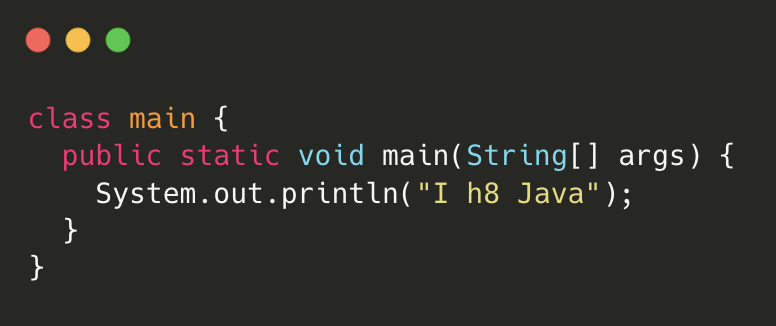
\includegraphics{misc/TITLEGRAPHIC.png}
        \end{figure}
        \vfill
        
        \small
        by Louis Meunier
        
        \href{https://notes.louismeunier.net}{\color{violet}{notes.louismeunier.net}}
        
    \end{center}
\end{titlepage}


{
  \hypersetup{linkcolor=violet}
  \tableofcontents
}

\newpage

\section{Quantum Theory and Atomic Structure}

\subsection{Electromagnetic Radiation}

\textbf{Light} can be described as a form of \textit{electromagnetic radiation}, meaning that it is a spectrum of wavelengths and corresponding frequencies. Classically, they are described as \textbf{waves}. What does this mean? 

A wave can be described as having the following properties:

\begin{itemize}
    \item \textbf{Wavelength} ($\lambda$): \textit{distance} traveled in a single cycle
    \item \textbf{Frequency} ($\nu$): the number of cycles per unit time. Standard units, \textit{Hz} ( = $s^{-1}$)
    \item \textbf{Amplitude}: half the height of the wave from \textit{peak} to \textit{trough}
    \item \textbf{Speed}: the \textit{distance} travelled per unit time of time. This can be expressed as $\lambda \nu$.
    
    Light (in a vacuum, which typically has to be assumed) has a standard speed, denoted $c \approx 2.998x10^{8} m/s$. Thus, we can write:
    
    $$c = \lambda \nu$$
    
    Since $c$ is a constant, we can state that if $\lambda$ increases, $\nu$ must decrease (and vice versa).
    \end{itemize}
    \subsection{Waves vs Particles}
    
    The distinction between the properties of waves and particles is very important in moving forward, as we will soon see. However, it is first and foremost important to be able to distinguish between the two.
    
    \begin{center}
        \begin{tabular}{ |c|c|c| } 
         \hline
         \textbf{Property} & \textbf{Waves} & \textbf{Particles} \\ 
         \hline
         Movement between media: & refract & slow, curve \\ 
         \hline
         Interaction with objects & bend, diffract & binary response: go through, or don't \\ 
         \hline
        \end{tabular}
    \end{center}

    It seems that waves and particles are very distinct, and yet early experiments showed some potential overlap between the two concepts, particularly in regards to light. 
    
    Experiments with light by people such as Planck showed that it did not always have respect classically-predicted trends when treated as a wave, particularly when it came to altering its frequency.
    
    \begin{figure}[!ht]%
        \centering
        \subfloat{{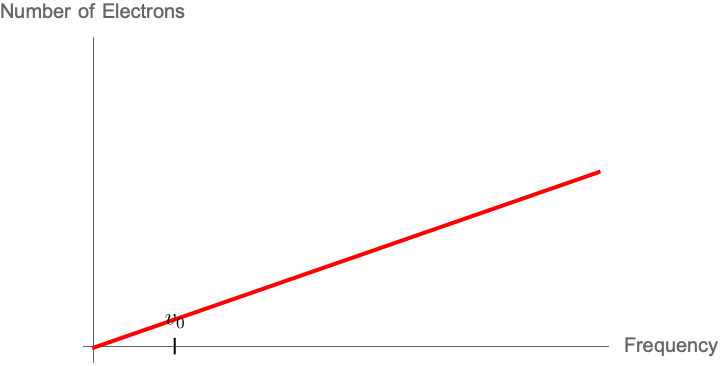
\includegraphics[width=6.5cm]{misc/numofelectronspredicted.png} }}%
        \qquad
        \subfloat{{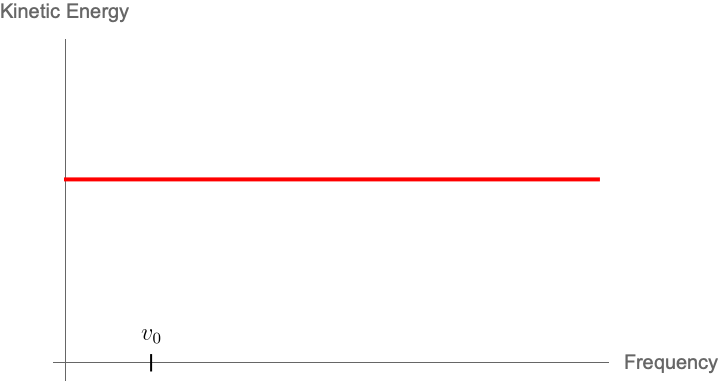
\includegraphics[width=6.5cm]{misc/kepredicted.png} }}%
        \caption{Predictions of the Properties of Light}
        \label{fig:experimentallight}%
    \end{figure}
    
    \begin{figure}[!ht]%
        \centering
        \subfloat{{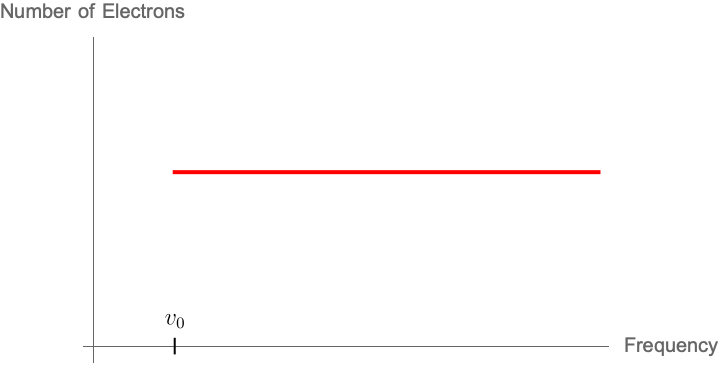
\includegraphics[width=6.5cm]{misc/numelectronsexperimental.png} }}%
        \qquad
        \subfloat{{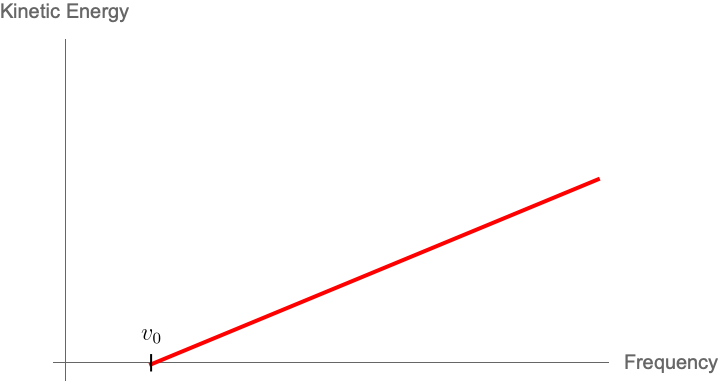
\includegraphics[width=6.5cm]{misc/keexperimental.png} }}%
        \caption{Experimental Properties of Light}
        \label{fig:experimentallight}%
    \end{figure}

    Further experiments lead to the idea of treating light as a \textit{photon} (think, a packet of energy) rather than a continuous wave. This idea came about from experiments with shining beams of light of varying brightness and frequency onto a metal plate; contrary to popular belief, the brightness had no effect on the number of electrons ejected from the plate. Instead the following formula was derived to explain the scenario:

    \begin{equation}
        \begin{split}
        E_{\text{photon}} &= \text{Kinetic Energy of Electron} + \text{Work Function}\\
        hv &= \frac{1}{2}m_e v_e^2 + \phi\\
        E &= \frac{1}{2}m_e v_e^2 + hv_0\\
        \end{split}
    \end{equation}

In this situation, $h$ is Planck's constant, $v$ is the frequency of the photon, $m_e$ is the mass of an electron, $v_e$ is the velocity of the electron, and $\phi$ is the work function of the metal (equal to $hv_0$, where $v_0$ is the threshold frequency needed to eject an electron from the metal).

Plank's constant ($h\approx 6.626x10^{-34} J \cdot s$) is a constant derived experimentally to define the ratio between energy and frequency; ie $E = hv (=\frac{hc}{\lambda})$.

\subsection{Atomic Spectra and Atomic Models}

\begin{figure}[!ht]
    \centering
    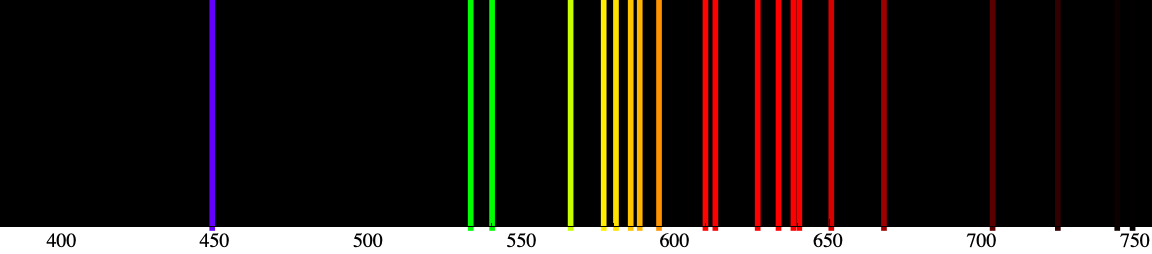
\includegraphics[width=7.5cm]{misc/neonatomicspectra.png}
    \caption{Atomic Spectra of Ne}
    \label{fig:atomicspectra}
\end{figure}

The atomic spectra, such as that picture in figure \ref*{fig:atomicspectra}, was, experimentally, found to be a unique pattern for each element when its electrons were excited. When this pattern was discovered, it disrupted current theories (such as Rutherford's atomic model, which involved electrons essentially filling any space around a central positive nucleus) of how the electron was structured, as these models would have implied a continuous, rather than discrete, atomic spectrum. 

Without a concrete explanation for this behavior, chemists instead tried to mathematically explain such behavior, leading to Rydberg's Equation:

\begin{equation*}
    \frac{1}{\lambda} = R\left(\frac{Z^2}{n_1^2}-\frac{Z^2}{n_2^2}\right)
\end{equation*}

Where $R$ is Rydberg's constant = $1.097x10^{7} m^{-1}$, $Z$ is the atomic number of the element in question, $n_1$ is the initial energy level of the electron, and $n_2$ is the final energy level of the electron. This model was developed using hydrogen, specifically, and is in fact only valid for "hydrogen-like" atoms (ie, atoms with a single electron in the outermost shell). This equation largely relied on Bohr's equation, which proposed that there exist particular states of energy for electrons in atoms, and that electrons can only exist in these states; think of rings of energy around the nucleus, and electrons can only exist in these rings.
\section{Electron Configuration and Chemical Periodicity}

\section{Models of Chemical Bonding}

\section{Shapes of Molecules}

\section{Theories of Covalent Bonding}

\section{Intermolecular Forces}


\end{document}